% !TEX TS-program = xelatex
% !BIB program = bibtex
% !TeX spellcheck = ru_RU

% About magic macros see also
% https://tex.stackexchange.com/questions/78101/

% По умолчанию используется шрифт 14 размера.
% Если Вы не влезаете в лимит страниц и нужен 12-й шрифт,
% то уберите опцию [14pt]
\documentclass[14pt, russian]{matmex-diploma-custom}

% !TeX spellcheck = ru_RU
% !TEX root = vkr.tex
% Опциональные добавления используемых пакетов. Вполне может быть, что они вам не понадобятся, но в шаблоне приведены примеры их использования.
\usepackage{tikz} % Мощный пакет для создание рисунков, однако может очень сильно замедлять компиляцию
\usetikzlibrary{decorations.pathreplacing,calc,shapes,positioning,tikzmark}

% Библиотека для TikZ, которая генерирует отдельные файлы для каждого рисунка
% Позволяет ускорить компиляцию, однако имеет свои ограничения
% Например, ломает пример выделения кода в листинге из шаблона
% \usetikzlibrary{external}
% \tikzexternalize[prefix=figures/]

\newcounter{tmkcount}

\tikzset{
    use tikzmark/.style={
            remember picture,
            overlay,
            execute at end picture={
                    \stepcounter{tmkcount}
                },
        },
    tikzmark suffix={-\thetmkcount}
}

\usepackage{booktabs} % Пакет для верстки "более книжных" таблиц, вполне годится для оформления результатов
% В шаблоне есть команда \multirowcell, которой нужен этот пакет.
\usepackage{multirow}
\usepackage{siunitx} % для таблиц с единицами измерений

\newcommand{\cd}[1]{\texttt{#1}}
\newcommand{\inbr}[1]{\left<#1\right>}

% Для названий стоит использовать \textsc{}
\newcommand{\OCaml}{\textsc{OCaml}}
\newcommand{\miniKanren}{\textsc{miniKanren}}
\newcommand{\BibTeX}{\textsc{BibTeX}}
\newcommand{\vsharp}{\textsc{V$\sharp$}}
\newcommand{\fsharp}{\textsc{F$\sharp$}}
\newcommand{\csharp}{\textsc{C\#}}
\newcommand{\GitHub}{\textsc{GitHub}}
\newcommand{\SMT}{\textsc{SMT}}

\newcolumntype{L}[1]{>{\raggedright\let\newline\\\arraybackslash\hspace{0pt}}m{#1}}
%\newcolumntype{C}[1]{>{\centering\let\newline\\\arraybackslash\hspace{0pt}}m{#1}}
\newcolumntype{R}[1]{>{\raggedleft\let\newline\\\arraybackslash\hspace{0pt}}m{#1}}

%  Команды и пакеты, не используемые в шаблоне, которые тем не менее могут быть полезными.

% \newcolumntype{Y}{>{\centering\arraybackslash}X}

% \usepackage{mathrsfs}

% \lstdefinelanguage{ocaml}{
% keywords={@type, function, fun, let, in, match, with, when, class, type,
% nonrec, object, method, of, rec, repeat, until, while, not, do, done, as, val, inherit, and,
% new, module, sig, deriving, datatype, struct, if, then, else, open, private, virtual, include, success, failure,
% lazy, assert, true, false, end},
% sensitive=true,
% commentstyle=\small\itshape\ttfamily,
% keywordstyle=\ttfamily\bfseries, %\underbar,
% identifierstyle=\ttfamily,
% basewidth={0.5em,0.5em},
% columns=fixed,
% fontadjust=true,
% literate={->}{{$\to$}}3 {===}{{$\equiv$}}1 {=/=}{{$\not\equiv$}}1 {|>}{{$\triangleright$}}3 {\\/}{{$\vee$}}2 {/\\}{{$\wedge$}}2 {>=}{{$\ge$}}1 {<=}{{$\le$}} 1,
% morecomment=[s]{(*}{*)}
% }

\usepackage{totcount}
\usepackage{setspace}

\definecolor{eclipseGreen}{RGB}{63,127,95}

\begin{document}
% TODO: Formatting
% !TeX spellcheck = ru_RU
% !TEX root = vkr.tex

%% Если что-то забыли, при компиляции будут ошибки Undefined control sequence \my@title@<что забыли>@ru
%% Если англоязычная титульная страница не нужна, то ее можно просто удалить.
\filltitle{ru}{
    %% Актуально только для курсовых/практик. ВКР защищаются не на кафедре а в ГЭК по направлению,
    %%   и к моменту защиты вы будете уже не в группе.
    chair              = {Кафедра системного программирования},
    group              = {21.Б10-мм},
    %
    %% Макрос filltitle ненавидит пустые строки, поэтому обязателен хотя бы символ комментария на строке
    %% Актуально всем.
    title              = {Оптимизация алгоритмов injected queue в рантайме Tokio},
    %
    %% Здесь указывается тип работы. Возможные значения:
    %%   production - производственная практика;
    %%   coursework - отчёт по курсовой работе (ОБРАТИТЕ ВНИМАНИЕ, у техпрога и ПИ нет курсовых, только практики);
    %%   practice - отчёт по учебной практике;
    %%   prediploma - отчёт по преддипломной практике;
    %%   master - ВКР магистра;
    %%   bachelor - ВКР бакалавра.
    type               = {bachelor},
    %
    %% Здесь указывается вид работы. От вида работы зависят критерии оценивания.
    %%   solution - «Решение». Обучающемуся поручили найти способ решения проблемы в области разработки программного обеспечения или теоретической информатики с учётом набора ограничений.
    %%   experiment - «Эксперимент». Обучающемуся поручили изучить возможности, достоинства и недостатки новой технологии, платформы, языка и т. д. на примере какой-то задачи.
    %%   production - «Производственное задание». Автору поручили реализовать потенциально полезное программное обеспечение.
    %%   comparison - «Сравнение». Обучающемуся поручили сравнить несколько существующих продуктов и/или подходов.
    %%   theoretical - «Теоретическое исследование». Автору поручили доказать какое-то утверждение, исследовать свойства алгоритма и т.п., при этом не требуя написания кода.
    kind               = {solution},
    %
    author             = {ЕРИН Игорь Антонович},
    %
    %% Актуально только для ВКР. Указывается код и название направления подготовки. Типичные примеры:
    %%   02.03.03 \enquote{Математическое обеспечение и администрирование информационных систем}
    %%   02.04.03 \enquote{Математическое обеспечение и администрирование информационных систем}
    %%   09.03.04 \enquote{Программная инженерия}
    %%   09.04.04 \enquote{Программная инженерия}
    %% Те, что с 03 в середине --- бакалавриат, с 04 --- магистратура.
    specialty          = {02.03.03 \enquote{Математическое обеспечение и администрирование информационных систем}},
    %
    %% Актуально только для ВКР. Указывается шифр и название образовательной программы. Типичные примеры:
    %%   СВ.5162.2020 \enquote{Технологии программирования}
    %%   СВ.5080.2020 \enquote{Программная инженерия}
    %%   ВМ.5665.2022 \enquote{Математическое обеспечение и администрирование информационных систем}
    %%   ВМ.5666.2022 \enquote{Программная инженерия}
    %% Шифр и название программы можно посмотреть в учебном плане, по которому вы учитесь.
    %% СВ.* --- бакалавриат, ВМ.* --- магистратура. В конце --- год поступления (не обязательно ваш, если вы были в академе/вылетали).
    programme          = {СВ.5162.2020 \enquote{Технологии программирования}},
    %
    %% Актуально всем.
    %% Должно умещаться в одну строчку, допускается использование сокращений, но без переусердствования,
    %% короткая строка с большим количеством сокращений выглядит странно
    %supervisorPosition = {проф. кафeдры системного программирования, д.ф.-м.н.,}, % Терехов А. Н.
    %supervisorPosition = {ст. преподаватель кафедры ИАС, к.~ф.-м.~н. (если есть),}, % Смирнов К. К.
    supervisorPosition = {Доцент кафедры системного программирования, к.ф.-м.н.,},
    supervisor         = {Гориховский~В.~И.},
    %
    %% Актуально только для практик и курсовых. Если консультанта нет или он совпадает с научником, закомментировать или удалить вовсе.
    consultantPosition = {Эксперт по разработке ПО, ООО ``Ядро Центр Программных Разработок'',},
    consultant         = {Ефремов~Р.~С.},
    %
    %% Актуально только для ВКР.
    reviewerPosition   = {Старший разработчик ПО, ООО ``Ядро Центр Программных Разработок'',},
    reviewer           = {Черепанов~А.~П.},
}
%
% Английский титульник нужен только для ВКР, остальные виды работ могут его смело игнорировать.
\filltitle{en}{
    chair              = {Advisor's chair},
    group              = {21.B10-mm},
    title              = {Optimization of injected queue algorithms in Tokio runtime},
    type               = {bachelor},
    author             = {Igor Erin},
    %
    %% Possible choices:
    %%   02.03.03 \foreignquote{english}{Software and Administration of Information Systems}
    %%   02.04.03 \foreignquote{english}{Software and Administration of Information Systems}
    %%   09.03.04 \foreignquote{english}{Software Engineering}
    %%   09.04.04 \foreignquote{english}{Software Engineering}
    %% Те, что с 03 в середине --- бакалавриат, с 04 --- магистратура.
    specialty          = {02.03.03 \foreignquote{english}{Software and Administration of Information Systems}},
    %
    %% Possible choices:
    %%   СВ.5162.2020 \foreignquote{english}{Programming Technologies}
    %%   СВ.5080.2020 \foreignquote{english}{Software Engineering}
    %%   ВМ.5665.2022 \foreignquote{english}{Software and Administration of Information Systems}
    %%   ВМ.5666.2022 \foreignquote{english}{Software Engineering}
    programme          = {СВ.5162.2020 \foreignquote{english}{Programming Technologies}},
    %
    %% Note that common title translations are:
    %%   кандидат наук --- C.Sc. (NOT Ph.D.)
    %%   доктор ... наук --- Sc.D.
    %%   доцент --- docent (NOT assistant/associate prof.)
    %%   профессор --- prof.
    supervisorPosition = {Sc.D, prof.},
    supervisor         = {V.~I.~Gorikhovskii},
    %
    consultantPosition = {Software Development Expert, OOO "Yadro Centr Programmnykh Razrabotok"},
    consultant         = {R.~S.~Efremov},
    %
    reviewerPosition   = {Software Senior Developer, OOO "Yadro Centr Programmnykh Razrabotok"},
    reviewer           = {A.~P.~Cherepanov},
}
%

\maketitle
\setcounter{tocdepth}{2}
\tableofcontents

% !TeX spellcheck = ru_RU
% !TEX root = vkr.tex

\section*{Введение}
\thispagestyle{withCompileDate}

\verb|TATLIN.BACKUP|\footnote{\href{https://yadro.com/ru/tatlin/backup}{TATLIN.BACKUP}
--- система хранения данных резервных копий (Дата обращения: 4.1.2025)} --- проект группы компаний \verb|YADRO|\footnote{\href{https://yadro.com/}{YADRO} --- официальный сайт компании (Дата обращения: 4.1.2025)}, посвященный созданию системы бекапов с использованием алгоритмов дедупликации написанный на языке \verb|Rust|. \verb|Rust| предоставляет \verb|async| / \verb|await|\cite{fsharpasyncawait} интерфейс для обработки асинхронных событий. Язык не фиксирует реализацию, позволяя пользователю выбирать асинхронный рантайм.

\verb|tokio|\footnote{\href{https://tokio.rs/}{tokio} --- официальный сайт проекта (Дата обращения: 4.1.2025)} --- проект, предоставляющий две реализации асинхронного рантайма: так называемые \verb|current_thread| и \verb|mutli_thread| рантаймы, частично реализует стандартную библиотеку языка с асинхронным интерфейсом, примитивы синхронизации, коллекции, таймеры, профилировщики --- одним словом целую экосистему для написания асинхронных программ.

Многопоточный рантайм из \verb|tokio| используется в \verb|TATLIN.BACKUP|, где был замечен недостаток текущей реализации: общая очередь асинхронный событий, разделяемая всеми потоками \verb|tokio|, защищена мьютексом и становится бутылочным горлышком по предположению инженеров из \verb|YADRO|.

Именно исследованию возможности улучшения производительности многопоточного рантайма \verb|tokio| в типичных для \verb|TATLIN.BACKUP| сценариях с помощью изменения алгоритмов общей очереди событий посвящена данная работа.

% !TeX spellcheck = ru_RU
% !TEX root = vkr.tex

\section{Постановка задачи}
\label{sec:task}

Целью данной работы является проверка гипотезы о бутылочном горлышке, коим явилась, по мнению команды \verb|TATLIN.BACKUP|, общая очередь асинхронных событий, и поиску решения этой проблемы. Для чего были поставлены следующие задачи:

\begin{enumerate}
    \item Создать воспроизводимую систему бенчмарков. Вероятно, совершенно искусственную, однако, позволяющую наблюдать сценарии взаимодействия с глобальной очередью.
    \item Произвести анализ собранных метрик. Удостовериться, что глобальная очередь действительно накладывает ограничение на производительность.
    \item Спроектировать решение. Алгоритм шедулинга, в том числе общая очередь, были созданы с оглядкой на реализацию в языке \verb|Go|. Необходимо проверить, что стало достигнуто там за это время.
    \item Прототипировать и анализировать полученные решения.
    \item Интегрировать решение.
\end{enumerate}

% !TeX spellcheck = ru_RU
% !TEX root = vkr.tex

\section{Обзор}

Данный раздел содержит обзор сущностей, взаимодейсвующих с глобальной очередью, метрик рантайма, инструментов бенчмаркинга.

\subsection{Многопоточный рантайм tokio}

При инстанциации рантайм создает определенное количество системных потоков для так называемого блокирующего пулла, призванного исполнять cpu bound задачи. Всего создается \verb|worker_threads| + \verb|max_blocking_threads| потков, где

\begin{itemize}
    \item \verb|worker_threads| --- количесво потоков предназначенных для исполенния асинхронных задач
    \item \verb|max_blocking_threads| --- максимальное количество блокирующих потоков
\end{itemize}

\begin{figure}[H]
    \begin{center}
        \makebox[\textwidth]{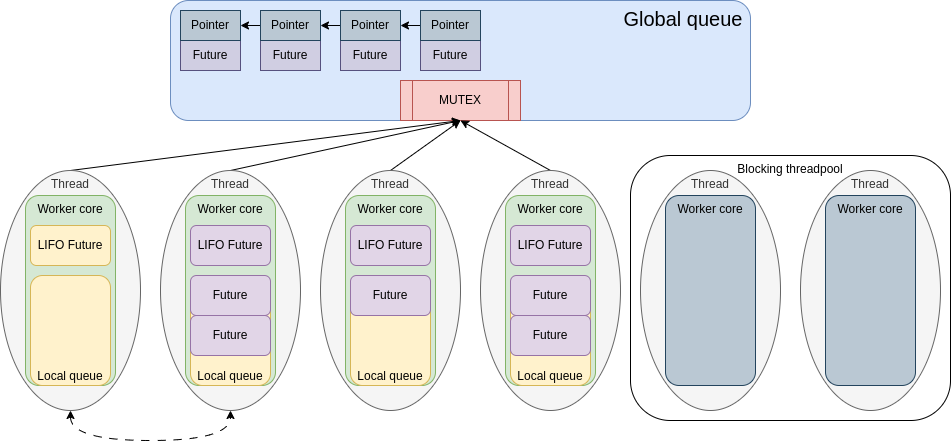
\includegraphics[scale=0.55]{pictures/tokio.arch.png}}
    \end{center}

    \caption{Упрощенное представление многопоточного рантайма}
    \label{fig:before}
\end{figure}

Блокирующие потоки ожидают определенный период, 10 секунд если не специфицировано иначе, поступления задач после чего прекращают свое исполнение.

\verb|Воркер|, так называется сущность ассоциированная с каждым из оставшихся \verb|worker_threads| потоков по средством размещения в локальной для этих поток переменной так называемого \verb|ядра воркера| --- структуры, необходимой для исполнения асинхронных задач, включающей \verb|локальную очередь|, хендлер \verb|глобальной очереди| и тому подобное.

\verb|Локальная очередь| воркера выступает в качестве кэша его задач, имеет фиксированный размер и предполагает добавление задач исключительно из потока владельца. Однако, изъятие из нее может быть осуществленно потоками других воркеров при нехватке оным собственных задач --- процесс называемый стилингом. Все это: фиксированный размер и производитель в единственном количестве позволяет ей иметь lock free алгоритм взаимодействия. В случае переполнения часть задач перемещается воркером в глобальную очередь.

\verb|Глобальная очередь| или \verb|inject queue| представляет собой коллекцию задач ожидающих исполнения. Наполняется она при спавнинге задачи вне контекста воркера или при переполеннии локальной очереди воркеров. Реализована с помощью интрузивного связного списка, защищенного мьютексом.

Исполнить асинхронное замыкание пользователь может несколькими способами:

\begin{itemize}
    \item \verb|block_on| --- метод инстанса рантайма позволяющий заблокировать поток приложения на исполнении определенного асинхронной задачи
    \item \verb|tokio::spawn| --- функция позволяющая поместить асинхронное замыкание в одну из очередей рантайма. Вызвов ее должен быть совершен в его контексте --- в одном из потоков, управляемых рантаймом, в методе \verb|block_on| или промежутке жизни объекта \verb|EnterGuard|. От места вызова будет зависеть, в какую очередь будет помещена задача: в случае потока воркер --- в локальную очередь, иначе --- глобальную
\end{itemize}

% TODO
\subsubsection{Выбор задачи}

Логика поиска воркером задачи для исполнения отражена на листинге \ref{listing:next_task}.

\begin{listing}
    \begin{minted}{rust}
fn next_task(&mut self) -> Option<Notified> {
    if self.tick % self.global_queue_interval == 0 {
        return next_remote_task()
                .or_else(|| self.next_local_task())
    }
    if Some(task) = self.next_local_task()  {
        return Some(task);
    }
    if inject().is_empty() {
        return None;
    }
    let (head, tail) = inject().pop_n(self.can_take());
    self.run_queue.push_back(tail);
    return head
}
    \end{minted}

    \caption{Логика выбора задачи}
    \label{listing:next_task}
\end{listing}

И осуществляется в следующем порядке: раз в определенное, конфигурируемое рантаймом, число тиков --- мера времени воркера, он пытается взять задачу из глобальной очереди, иначе --- из локальной, в остальное время проверяется локальная, после глобальная очереди.

\subsection{Цикл работы воркера}

Алгоритм рабочего цикла воркера отражен на листинге \ref{listing:worker:run}.

\begin{listing}
    \begin{minted}{rust}
fn run() {
    while !is_shutdown() {
        core.tick();
        if let Some(task) = core.next_task() {
            self.run_task(task, core);
            continue;
        }
        if let Some(task) = core.steal_work() {
            self.run_task(task, core);
            continue;
        }
        self.park(core)
    }
}
    \end{minted}

    \caption{Логика выбора следующей задачи}
    \label{listing:worker:run}
\end{listing}

А именно, воркер отсчиты тик, затем пытается взять найти задачу, после чего пытается украсть задачи у других воркеров. В случае неудачи он паркует поток.

\subsection{Метрики}

Метрики собираемые рантаймом предполагается использовать в двух направлениях:

\begin{itemize}
    \item Семплирование --- наблюдения поведения внутренних структур рантайма в определенный моменты исполнения задач
    \item Тотальная оценка --- анализ количеств тех или иных операций произведенных за весь период исполнения
\end{itemize}

К первому типу можно отнести глубину глобальной или локальных очередей в определенный момент времени. К последнему --- количество переполнений локальных очередей за все время исполнения. Стоит отметить, что количество переполнений без сомнений имеет смысл фиксировать и во время исполнения определенных сценариев, однако, семплинг не точен и с легкостью может упустить стремительно меняющиеся значения. Тогда как тотальная сумма не позволяет упускать отдельные опреции.

\verb|tokio-metrics| --- проект, предоставющий интерфейс для семплирования метрик рантайма. Далее будет представлен полный перечень метрик доступных из \verb|tokio-metrics|. Метрики будут разбиты на группы по аналогии для уменьшения повторений.

Группа предполагает перечисление в следующем порядке: значение представленное в tokio-metrics как общее значение для всех воркеров, минимум и максимум среди воркеров, оданко, для краткости в тексте будут обзоначены только именования суммарных.

\begin{itemize}
    \item \verb|total_park_count| --- количество парковок потоков воркеров
    \item \verb|mean_poll_duration| --- это значение представляет собой экспоненциально взвешенную скользящую среднюю продолжительности опросов задач
    \item \verb|total_noop_count| --- сколько раз поток воркера был распаркован, но не совершил никакой работы перед парковкой
    \item \verb|total_steal_count| --- количество задач, которые воркеры похитили, перместив их в свою локальную очередь
    \item \verb|total_steal_operations| --- количесво раз воркеры успешно похител задачи
    \item \verb|total_local_schedule_count| --- количество задач отправленных на исполенние из контектса воркера, что должна попасть в одну из локальных очередей
    \item \verb|total_overflow_count| --- сколько раз воркеры переполнили свои локальные очереди
    \item \verb|total_polls_count| --- количество опросов задач среди
    \item \verb|total_busy_duration| --- количество времени исполения задач
    \item \verb|total_local_queue_depth| --- количество задач помещенных в локальные очереди
\end{itemize}

И остальные:

\begin{itemize}
    \item \verb|workers_count| --- количество воркеров исполняющих задачи. Значение специфицируется при инстанциации рантайма

    \item \verb|poll_time_histogram| --- гистограмма опросов задач, сгруппированная по времени исполнения опросов

    \item \verb|num_remote_schedules| --- количество задач, отправленных на исполнение из вне. То есть количество задачи заспавненных вне контекста воркера, задач, попавших в глобальную очередь

    \item \verb|global_queue_depth| --- количество задач, помещенных в глобальную очередь
\end{itemize}

Для решения поставленных задач были выделены метрики, отражающие взаимодействие воркеров с очередями. То есть, метрики, демонстрирущие глубину глобальной очереди (\verb|global_queue_depth|), локальных очередей (\verb|total_local_queue_depth|), количество переполнений (\verb|total_overflow_count|), количество похищенных задач (\verb|total_steal_count|), количество удаленных спавнов (\verb|num_remote_schedules|).

\subsection{Бенчмаркинг}

Для измерений времени исполнения и пропускной способности была использована библиотека \verb|criterion|\footnote{\href{https://github.com/bheisler/criterion.rs}{Репозиторий} проекта criterion}. Так как она популярна, имеет обширную документацию, использовуется в \verb|tokio|.

\subsection{Изменения шедулера языка Go}

Как было отмечено ранее, алгоритмы шедулинга в tokio были созданы с оглядкой на реализацию рантайма языка Go. В свою очередь шедулинг корутин в Kotlin был сделать по мотивам tokio. С тех пор, никаких изменений рантайм Go не претерпел, точно так же, как рантайм языка Kotlin. Таким образом, все рантаймы предопологают наличия локальных очередей у воркеров и одной глобальной очереди с взаимноисключающим владением.

% !TeX spellcheck = ru_RU
% !TEX root = vkr.tex

\section{Описание решения}

\subsection{Метрики}

Метрики собираемые рантаймом предполагается использовать в двух направлениях:

\begin{itemize}
    \item Семплирование --- наблюдения поведения внутренних структур рантайма в определенный моменты исполнения задач
    \item Тотальная оценка --- анализ количеств тех или иных операций произведенных за весь период исполнения
\end{itemize}

К первому типу можно отнести глубину глобальной или локальных очередей в определенный момент времени. К последнему --- количество переполнений локальных очередей за все время исполнения. Стоит отметить, что количество переполнений без сомнений имеет смысл фиксировать и во время исполнения определенных сценариев, однако, семплирование с легкостью может упустить стремительно меняющиеся значения. Тогда как тотальная сумма не позволяет упускать отдельные операции.

\verb|tokio-metrics|\footnote{\href{https://github.com/tokio-rs/tokio-metrics}{Репозиторий} проекта tokio-metrics (Дата обращения: 4.1.2025)} --- проект, предоставляющий интерфейс для семплирования метрик рантайма. Далее будет представлен полный перечень метрик доступных из \verb|tokio-metrics|. Метрики будут разбиты на группы по аналогии для уменьшения повторений.

Группа предполагает перечисление в следующем порядке: значение представленное в \verb|tokio-metrics| как общее значение для всех воркеров, минимум и максимум среди воркеров, однако, для краткости в тексте будут обозначены только первое.

\begin{itemize}
    \item \verb|total_park_count| --- количество парковок потоков воркеров
    \item \verb|mean_poll_duration| --- это значение представляет собой экспоненциально взвешенную скользящую среднюю продолжительности опросов задач
    \item \verb|total_noop_count| --- сколько раз поток воркера был распаркован, но не совершил никакой работы перед парковкой
    \item \verb|total_steal_count| --- количество задач, которые воркеры похитили, переместив их в свою локальную очередь
    \item \verb|total_steal_operations| --- количество раз воркеры успешно похитили задачи
    \item \verb|total_local_schedule_count| --- количество задач отправленных на исполнение из контекста воркера, что должны попасть в одну из локальных очередей
    \item \verb|total_overflow_count| --- сколько раз воркеры переполнили свои локальные очереди
    \item \verb|total_polls_count| --- количество опросов задач
    \item \verb|total_busy_duration| --- количество времени исполнения воркерами задач
    \item \verb|total_local_queue_depth| --- количество задач помещенных в локальные очереди
\end{itemize}

И остальные:

\begin{itemize}
    \item \verb|workers_count| --- количество воркеров исполняющих задачи. Значение специфицируется при инстанциации рантайма

    \item \verb|poll_time_histogram| --- гистограмма опросов задач, сгруппированная по времени исполнения опросов

    \item \verb|num_remote_schedules| --- количество задач, отправленных на исполнение из вне. То есть количество задач, попавших в глобальную очередь при создании

    \item \verb|global_queue_depth| --- количество задач, помещенных в глобальную очередь
\end{itemize}

Для решения поставленных задач были выделены метрики, отражающие взаимодействие воркеров с очередями. То есть, метрики, демонстрирующие глубину глобальной очереди (\verb|global_queue_depth|), локальных очередей (\verb|total_local_queue_depth|), количество переполнений (\verb|total_overflow_count|), количество похищений (\verb|total_steal_operations|), количество удаленных спавнов (\verb|num_remote_schedules|).

Стоит отметить возможность сбора метрик для отдельной задачи, применение чему не было найдено.

\subsection{Система бенчмарков}

В качестве системы бенчмарков был создан проект \verb|tokiobench|\footnote{\href{https://github.com/IgorErin/tokiobench}{Репозиторий} проект tokiobench (Дата обращения: 4.1.2025)}, где предполагалось реализовать автоматизированные сценарии бенчмарков, сбор метрик и визуализацию полученных данных в виде графиков.

\subsection{Поиск сценариев}

В условиях недоступности кода \verb|TATLIN.BACKUP| поиск интересных с точки зрения производительности сценариев по взаимодействию с глобальной очередью был начат с репозиторий проекта \verb|tokio|.

Среди приведенных там сценариев был выделен один, представленный на листинге \ref{listing:bench:tokio:remote}.

\begin{listing}[H]
    \begin{minted}{rust}
for _ in 0..NUM_SPAWN {
    handles.push(rt.spawn(async {}));
}
rt.block_on(async {
    for handle in handles.drain(..) {
        handle.await.unwrap();
    }
});
    \end{minted}

    \caption{Tokio context spawning benchmark}
    \label{listing:bench:tokio:remote}
\end{listing}

А именно, задачи, в виде пустых асинхронных замыканий, спавнятся в главном потоке, их хендлеры коллекционируются, после чего рантайм поочередно ожидает исполнения задач используя метод \verb|block_on|.

В ходе общения с инженерами из \verb|TATLIN.BACKUP| был выделен сценарий их приложения: там присутствуют задачи, далее именуемые спавнерами, которые создают множество простых задач, далее именуемых листовыми задачами. Причем количество спавнеров и листовых задач варьируется.

\subsection{Проблема синхронизации}

Измерение производительности в данном случае предполагает измерение пропускной способности рантайма, что подразумевает измерение времени необходимое этому рантайму для исполнения фиксированного количества задач. Однако, для этого необходимо определить, когда все задачи были исполнены. Публичный интерфейс \verb|tokio| не позволяет получить информацию об этом, так как число необходимых к исполнению задач известно лишь пользователю. То есть нужно иметь какую-то синхронизацию, блокировать поток бенчмарка в ожидании конца обработки специфицированных рантайму задач. В бенчмарках \verb|tokio| делают это следующими способами:

\begin{itemize}
    \item Коллекционирует хендлеры, как представлено на листинге \ref{listing:bench:tokio:remote} и последовательно ожидают их в цикле с помощью метода \verb|block_on|
    \item Создают атомарную переменную с значением равным количеству задач и в каждой листовой задаче уменьшают ее значение на единицу. Задача, которая получила ноль в результате операции атомарного декремента, посылает сигнал с помощью блокирующего канала в главный поток, тем самым разблокирует его, как представлено на листинге \ref{listing:bench:tokio:atom}
\end{itemize}

\begin{listing}[H]
    \begin{minted}{rust}
let (tx, rx) = mpsc::sync_channel(1000);
let rem = Arc::new(AtomicUsize::new(NUM_SPAWN));

rt.block_on(async {
    for _ in 0..NUM_SPAWN {
        let tx = tx.clone();
        let rem = rem.clone();
        tokio::spawn(async move {
            if 1 == rem.fetch_sub(1, Relaxed) {
                tx.send(()).unwrap();
            }
        });
    }
    rx.recv().unwrap();
});
    \end{minted}

    \caption{Атомарная синхронизация в бенчмарках tokio}
    \label{listing:bench:tokio:atom}
\end{listing}

Такой дизайн имеет несколько явных недостатков:

\begin{itemize}
    \item Атомарное чтение и запись из множества исполняемых разными потоками задач скорее позволяет измерять производительность системы памяти физической машины, нежели взаимодействия структур рантайма
    \item Ожидание исполнения в методе \verb|block_on| чревато неточным измерением из-за текущей реализации\footnote{\href{https://github.com/bheisler/criterion.rs/issues/819}{Проблема} измерения производительности асинхронных функций (Дата обращения: 4.1.2025)}
\end{itemize}

Эти методы были улучшены:

\begin{itemize}
    \item Атомарные переменная была заменена иерархией заранее аллоцированных переиспользуемых от итерации к итерации буферами коллекционирующими хендлеры задач
    \item Ожидание хендлеров задач перенесено в отдельную задачу, которая сообщает о завершении обработки с помощью блокирующего канала
\end{itemize}

% !TeX spellcheck = ru_RU
% !TEX root = vkr.tex

\section{Эксперимент}
% !TeX spellcheck = ru_RU
% !TEX root = vkr.tex

\section{Заключение}

В ходе работы были выполнены следующие задачи:

\begin{itemize}
    \item Получено первое описание реализации tokio с точки зрения асинхронного интерфейса языка \verb|Rust|. В результате обзора выявлены две возможные уязвимости с точки зрения производительности: взаимодействие исполнителей и реализация глобальной очереди. Первая уязвимость была устранена в результате текущей работы путем шардирования планировщика многопоточного рантайма. Изменение многопоточного рантайма с точки зрения алгоритмов глобальной очереди рассмотрены в ВКР Матвея Калашникова: ``Оптимизация системы управления очередью задач в библиотеке Tokio для асинхронного рантайма''.
    \item Создан проект, содержащий бенчмарки, позволяющий автоматически собирать метрики и визуализировать результаты\footnote{\href{https://github.com/IgorErin/tokiobench}{Репозиторий} проект tokiobench (Дата обращения: 25.5.2025)}.
    \item Произведен эксперимент, основанный на ключевом сценарии использования \verb|tokio| в \verb|TATLIN.BACKUP|. Обнаружена возможность увеличить пропускную способность \verb|TATLIN.BACKUP|, что может свидетельствовать о существовании ограничения, накладываемого глобальной очередью. Однако, такой подход остается небезопасным.
    \item Предложена и реализована безопасная модификация рантайма, позволяющая использовать несколько глобальных очередей в одном инстансе рантайма\footnote{\href{https://github.com/IgorErin/tokio/pull/3}{Реализация} шардирования многопоточного рантайма. Имя пользователя: IgorErin (Дата обращения: 25.5.2025)}.
    \item Проведены эксперименты на целевом сценарии \verb|TATLIN.BACKUP|, показавшие увеличение производительности предложенного решения.
\end{itemize}

Языковые асинхронные интерфейсы трудны в создании вследствие необходимости наличия высокопроизводительной реализации для различных сред: будь то приложения для встроенных систем~\cite{CPPCoroutinesOnMicrocontrollers, AsyncIOT} или пользовательские программные продукты, способные эффективно исполняться на различных архитектурах и операционных системах~\cite{CPPCoroutinesDesignAndImpl}.

Известно множество исследований, направленных на изучение создания и оптимизации пуллов для исполнения вычислительных задач~\cite{ThreadPoolSize, PerfDeviationsInThreadPools, SyncInThreadPools, ProduserConsumerThreadPool}. Однако автору не удалось найти академические работы, посвященные реализации языковым асинхронных рантаймов. Вероятно, это связано с относительно недавним их появлением в языках с повышенным контролем над ресурсами~\cite{CPPCoroutinesDesignAndImpl}.

Стоит отметить, что асинхронные движки таких популярных языков, как Go, Kotlin, tokio в экосистеме языка Rust представляют собой вариации дизайна, предложенного Дмитрием Вьюковым для языка Go~\cite{GoScheduler, GoSchedulerImpropvements}. Данная работа показывает, что незначительные изменения в этом популярном подходе могут увеличить пропускную способность отдельных бенчмарков на порядок, что может свидетельствовать о необходимости дальнейших исследований использования современных асинхронных интерфейсов~\cite{ModernStorageAPI} и подходов к многопоточности~\cite{ThreadPerCore}.


\setmonofont{CMU Typewriter Text}
\bibliographystyle{ugost2008ls}
\bibliography{vkr}

\end{document}
